\documentclass[10pt,a4paper,twocolumn]{article}

% ------------------------------------------------------------------ IEEE-like layout
\usepackage[a4paper,top=19mm,bottom=24mm,left=16mm,right=16mm,columnsep=6mm]{geometry}
\usepackage{amsmath,amssymb,bm}
\usepackage{mathptmx}
\usepackage[no-math]{fontspec}
\setmainfont{TeX Gyre Termes}
\usepackage{polyglossia}
\setmainlanguage{english}
\usepackage{graphicx,booktabs,multirow,array}
\usepackage[table]{xcolor}
\usepackage{tikz}
\usetikzlibrary{positioning,arrows.meta,fit,backgrounds,calc,decorations.pathreplacing,shapes.geometric}
\usepackage{caption}
\usepackage{subcaption}
\usepackage{titlesec}
\usepackage{enumitem}
\usepackage[most]{tcolorbox}
\usepackage{fancyhdr}
\usepackage{stfloats}
\usepackage[colorlinks=true,linkcolor=black,citecolor=black,urlcolor=cBlue]{hyperref}

\definecolor{cBlue}{HTML}{2A78D6}
\definecolor{cOrange}{HTML}{EB6834}
\definecolor{cAqua}{HTML}{1BAF7A}
\definecolor{cYellow}{HTML}{EDA100}
\definecolor{cMagenta}{HTML}{E87BA4}
\definecolor{cViolet}{HTML}{6250D6}
\definecolor{cInk}{HTML}{0B0B0B}
\definecolor{cInk2}{HTML}{52514E}
\definecolor{cGrid}{HTML}{E4E3DF}
\definecolor{cPale}{HTML}{F3F6FB}

\renewcommand\thesection{\Roman{section}}
\renewcommand\thesubsection{\Alph{subsection}}
\renewcommand\thesubsubsection{\arabic{subsubsection})}
\titleformat{\section}{\centering\normalsize\scshape}{\thesection.}{0.5em}{}
\titleformat{\subsection}{\normalsize\itshape}{\thesubsection.}{0.5em}{}
\titleformat{\subsubsection}[runin]{\normalsize\itshape}{\thesubsubsection}{0.4em}{}[:]
\titlespacing*{\section}{0pt}{8pt}{4pt}
\titlespacing*{\subsection}{0pt}{6pt}{3pt}
\titlespacing*{\subsubsection}{\parindent}{3pt}{0.5em}

\renewcommand\thetable{\Roman{table}}
\captionsetup{font=footnotesize,labelsep=period,justification=justified,singlelinecheck=true}
\captionsetup[figure]{name=Fig.}
\captionsetup[table]{name=TABLE,labelsep=newline,justification=centering,font={footnotesize,sc}}
\setlength{\abovecaptionskip}{4pt}
\setlength{\textfloatsep}{8pt}
\setlength{\dbltextfloatsep}{8pt}
\setlist{nosep,leftmargin=*}

\newtcolorbox{keypoint}[1][Key point]{enhanced,breakable,colback=cPale,colframe=cBlue,
  boxrule=0.4pt,arc=1pt,left=3pt,right=3pt,top=2pt,bottom=2pt,fonttitle=\footnotesize\bfseries,
  coltitle=white,title=#1,fontupper=\footnotesize}

\pagestyle{fancy}
\fancyhf{}
\fancyhead[C]{\footnotesize\textsc{Spatio-Temporal 5G QoS Forecasting from Real Network Measurements}}
\fancyfoot[C]{\footnotesize\thepage}
\renewcommand{\headrulewidth}{0pt}

\newcommand{\x}{\bm{x}}
\newcommand{\p}{\bm{p}}
\newcommand{\R}{\mathbb{R}}

\begin{document}

% ================================================================== TITLE
\twocolumn[{%
\begin{center}
{\LARGE Spatio-Temporal 5G QoS Forecasting from Real Network\\[2pt]
Measurements, with Real-Time Monitoring}\\[10pt]
{\large Sabrine Assili}\\[2pt]
{\small National School of Electronics and Telecommunications of Sfax (ENET'Com), Tunisia\\
Source code: \href{https://github.com/Sabrine74/5g-spatiotemporal-qos-forecasting}{\texttt{github.com/Sabrine74/5g-spatiotemporal-qos-forecasting}}\\
LinkedIn: \href{https://www.linkedin.com/in/sabrineassili74/}{\texttt{linkedin.com/in/sabrineassili74}}}\\[10pt]
\end{center}
\begin{minipage}{\textwidth}
\small\bfseries\itshape
Abstract\,---\,\normalfont\bfseries
Applications such as adaptive video streaming and connected vehicles need to know the
quality of service (QoS) a mobile network will deliver \emph{in the next seconds}, not only
the current one. We study short-term downlink throughput forecasting on real measurements
from a commercial 5G network (21 traces, 45,768 seconds, driving and static), using
four groups of information available at time~$t$: throughput history, radio channel
indicators, mobility (speed, Doppler shift, handovers) and space (position and a
space-time throughput prior learned from other drives). With a leakage-free protocol that
holds out entire traces, a gradient-boosted model (LightGBM) beats the persistence baseline
in every fold, reducing the error of the mean throughput over the next 1, 3 and 5\,s by
3, 16 and 25\,\% (MAE) and 15, 25 and 30\,\% (RMSE). An ablation study shows that, on
average, history carries almost all the predictive information; radio and mobility features
help only where history fails, right after handovers, where they turn a model worse than
persistence into one 3\,\% better. The space-time prior does not improve accuracy on this
dataset, and normalised error does not grow with speed, which we explain with channel
coherence time. Conformalised quantile regression gives 80\,\% prediction intervals with
78\,\% empirical coverage on unseen drives (72\,\% without calibration). In a trace-driven
video-streaming simulation, using the forecast instead of the classic harmonic-mean
estimator raises the quality of experience on 19 of 21 traces. Finally, we package the
model as a real-time monitoring system (FastAPI, InfluxDB, Grafana) with predictive alerts.
\\[6pt]
\small\bfseries\itshape Index Terms\,---\,\normalfont\bfseries
5G, QoS prediction, predictive QoS, throughput forecasting, spatio-temporal data,
handover, Doppler, conformal prediction, adaptive video streaming, Grafana.
\end{minipage}
\vspace{12pt}
}]

% ================================================================== I
\section{Introduction}

The throughput of a mobile connection changes from second to second: the radio channel
fades, the user moves between cells, and other users share the same cell. Many applications
would behave better if they knew this throughput \emph{a few seconds in advance}. A video
player could pick the right quality before a drop instead of stalling; a connected car could
lower the resolution of its sensor stream before entering a coverage hole; a remote driving
session could slow down the vehicle in time. This idea is called \emph{predictive QoS}: the
automotive industry has identified it as a key enabler of 5G-connected
vehicles~\cite{5gaa}, and 3GPP has standardised a network data analytics function (NWDAF)
that exposes QoS predictions to applications~\cite{nwdaf}.

Forecasting throughput from measurements is an old problem in 4G~\cite{linkforecast} and
has been studied for commercial mmWave 5G~\cite{lumos5g}. Three questions remain open for
a practitioner who wants to build such a system on real data:
\begin{itemize}
\item \textbf{Q1 -- Accuracy.} Can a learned model beat the trivial forecast ``the next
seconds will look like now'' (\emph{persistence}) on drives it has never seen?
\item \textbf{Q2 -- Information.} What helps beyond past throughput: radio indicators,
mobility (speed, Doppler, handovers), or the \emph{location} of the user, i.e.\ a
spatio-temporal (``4D'': position + time) view of QoS?
\item \textbf{Q3 -- Usefulness.} Can the forecast come with a reliable uncertainty, and does
it improve a real application?
\end{itemize}

This work answers these questions on a public dataset collected on a commercial 5G
network~\cite{raca2020}. Its \textbf{contributions} are:
\begin{enumerate}
\item a leakage-free forecasting protocol on real 5G traces (whole drives held out,
validity mask on gaps), with naive baselines that a model must beat;
\item an ablation of four feature groups, including physically motivated mobility
features (Doppler shift, handovers) and a space-time throughput prior evaluated at the
position the vehicle will reach in $h$ seconds;
\item calibrated 80\,\% prediction intervals by conformalised quantile regression;
\item a trace-driven video-streaming evaluation of the forecast's practical value;
\item an open-source real-time monitoring stack (FastAPI, InfluxDB, Grafana) with
predictive alerts.
\end{enumerate}

Section~\ref{sec:data} presents the dataset, Section~\ref{sec:method} the method and
Section~\ref{sec:system} the real-time system. Section~\ref{sec:results} reports the
results, Section~\ref{sec:discussion} discusses them and Section~\ref{sec:conclusion}
concludes.

% ================================================================== II
\section{Dataset}
\label{sec:data}

\subsection{Source}
We use the 5G production dataset of Raca~\textit{et al.}~\cite{raca2020}, collected in
Cork, Ireland, between December~2019 and February~2020 on the network of a major Irish
operator. A phone running the G-NetTrack Pro application logged, about once per second,
the GPS position and speed, the serving cell, the radio technology (5G, LTE or 3G), the
channel indicators RSRP, RSRQ, SNR, CQI and RSSI (plus RSRP/RSRQ of the 5G NR carrier) and
the downlink throughput. The 5G network is non-standalone (NSA): 5G radio anchored on a
4G core, the architecture deployed by operators at the time.

\subsection{Which traces measure the network?}
The dataset has three applications (Table~\ref{tab:apps}). In the two video-streaming
applications, the measured throughput is mostly set by the video player, not by the
network: once its buffer is full, the player stops downloading, and 74\,\% of Netflix
seconds show zero throughput. Forecasting these values would mean forecasting the player.
We therefore keep the 21 \emph{file-download} traces, during which the phone downloads
continuously and the measured throughput approximates the capacity offered by the
network (only 3.8\,\% zero seconds).

\begin{table}[t]
\caption{Applications in the dataset}
\label{tab:apps}
\centering\footnotesize
\begin{tabular}{@{}lrrrr@{}}
\toprule
Application & Traces & Samples & Zero thr. & Median (Mbit/s) \\
\midrule
\textbf{File download (kept)} & 21 & 43,208 & 3.8\,\% & 12.1 \\
Netflix & 33 & 72,832 & 73.7\,\% & 0.0 \\
Amazon Prime & 29 & 72,671 & 37.6\,\% & 0.3 \\
\bottomrule
\end{tabular}
\end{table}

\subsection{Cleaning}
Each trace is put on a regular 1-second grid: rows sharing a timestamp are averaged, and
gaps of up to 3\,s are filled forward (14.9\,\% of grid seconds). Filled seconds are used
to compute features but never as evaluation targets (Section~\ref{sec:protocol}). Values
outside the 3GPP reporting ranges, such as Android's ``unavailable'' code $2^{31}-1$ or
RSRP~$=-200$\,dBm, are set to missing. The result has 45,768 seconds
(Table~\ref{tab:stats}). Driving and static conditions differ strongly
(Fig.~\ref{fig:dist}): the static sites were all served by 5G, with a median of 36\,Mbit/s,
while driving combines 5G, LTE and 3G with a median of 9\,Mbit/s and 686 cell changes.
Fig.~\ref{fig:map} shows the routes and how throughput varies along them.

\begin{table}[t]
\caption{File-download traces after cleaning}
\label{tab:stats}
\centering\footnotesize
\setlength{\tabcolsep}{3.5pt}
\begin{tabular}{@{}lrrrrrr@{}}
\toprule
 & Traces & Seconds & \multicolumn{2}{c}{Thr.\ (Mbit/s)} & 5G & Cell \\
\cmidrule(lr){4-5}
 & & & median & p90 & share & changes \\
\midrule
Driving & 16 & 28,551 & 9.0 & 96.8 & 51\,\% & 686 \\
Static & 5 & 17,217 & 36.1 & 205.0 & 100\,\% & 0 \\
\bottomrule
\end{tabular}
\end{table}

\begin{figure}[t]
\centering
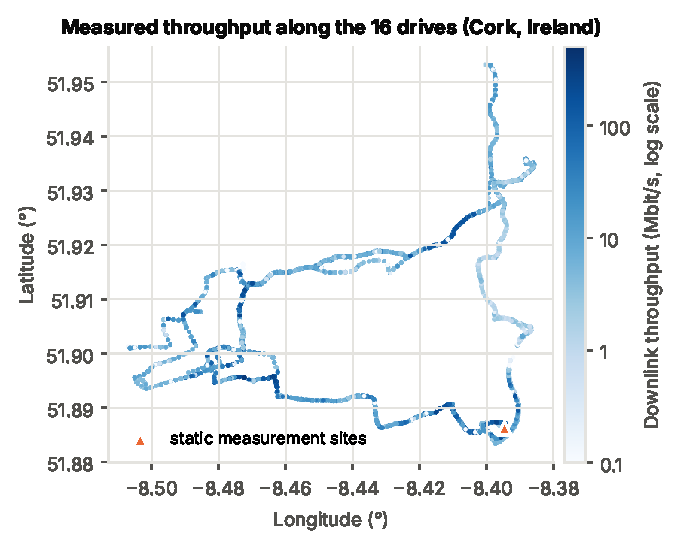
\includegraphics[width=0.92\columnwidth]{fig/fig_map.pdf}
\caption{Routes of the 16 drives, coloured by measured throughput (log scale), and the
five static sites. Throughput varies along the routes, which motivates a spatial view.}
\label{fig:map}
\end{figure}

\begin{figure}[t]
\centering
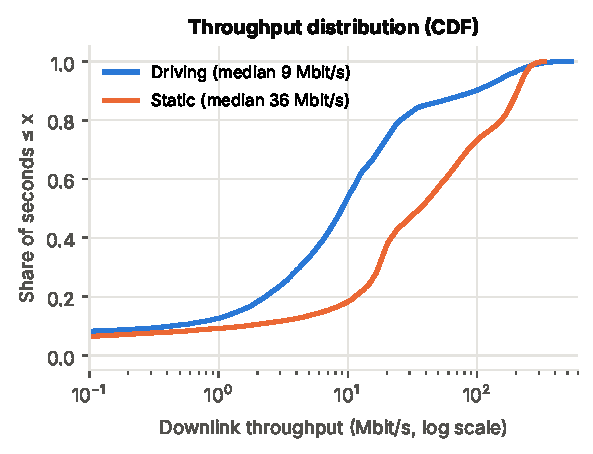
\includegraphics[width=0.8\columnwidth]{fig/fig_distribution.pdf}
\caption{Cumulative distribution of throughput. The distribution is heavy-tailed (0 to
533\,Mbit/s) and four times higher when static than when driving.}
\label{fig:dist}
\end{figure}

% ================================================================== III
\section{Method}
\label{sec:method}

\begin{figure*}[t]
\centering
\begin{tikzpicture}[font=\scriptsize, node distance=4mm and 5mm,
  stage/.style={draw=cInk2, rounded corners=2pt, fill=white, align=left, inner sep=3pt, text width=#1},
  stage/.default=27mm,
  arr/.style={-{Stealth[length=2.2mm]}, thick, cInk2}]
\node[stage=24mm] (data) {\textbf{1. Measurements}\\[1pt]
  21 download traces\\ 1-s grid, 45,768 s\\ KPIs + GPS + speed\\ + cell + technology};
\node[stage=50mm, right=of data, draw=cBlue, fill=cPale] (feat) {\textbf{2. Features at time $t$} (past only)\\[1pt]
  \textcolor{cBlue}{$\blacksquare$} \textbf{history}: lags, rolling stats, EWMA\\
  \textcolor{cAqua}{$\blacksquare$} \textbf{radio}: RSRP, RSRQ, SNR, CQI, trends\\
  \textcolor{cMagenta}{$\blacksquare$} \textbf{mobility}: speed, Doppler $f_D$, handovers\\
  \textcolor{cOrange}{$\blacksquare$} \textbf{space}: position, prior at $\p_t$ and $\hat\p_{t+h}$\\
  target: mean throughput over $(t, t{+}h]$};
\node[stage=31mm, right=of feat, yshift=7mm] (mod) {\textbf{3a. Point forecast}\\[1pt]
  persistence, harmonic mean,\\ ridge, MLP, \textbf{LightGBM}\\ $h \in \{1, 3, 5\}$\,s};
\node[stage=31mm, below=3mm of mod] (unc) {\textbf{3b. Uncertainty}\\[1pt]
  quantile LightGBM\\ + conformal calibration (CQR)};
\node[stage=36mm, right=of mod, yshift=-7mm] (eval) {\textbf{4. Evaluation}\\[1pt]
  5-fold CV, whole traces held out\\ MAE, RMSE, skill vs persistence\\ ablation, speed, handovers\\ coverage, video-streaming QoE};
\draw[arr] (data) -- (feat);
\draw[arr] (feat.east) -- ++(2.5mm,0) |- (mod.west);
\draw[arr] (feat.east) -- ++(2.5mm,0) |- (unc.west);
\draw[arr] (mod.east) -- ++(2.5mm,0) |- (eval.west);
\draw[arr] (unc.east) -- ++(2.5mm,0) |- (eval.west);
\end{tikzpicture}
\caption{Forecasting pipeline. All features at time $t$ use only data measured up to $t$;
the space-time prior is learned inside each fold from the training drives only.}
\label{fig:pipeline}
\end{figure*}

\subsection{Problem formulation}
For trace $i$ and second $t$, let $r_t$ be the measured downlink throughput. Given the
features $\x_t$ available at time $t$, we forecast the \emph{mean throughput over the next
$h$ seconds}:
\begin{equation}
y_{t,h}=\frac{1}{h}\sum_{k=1}^{h} r_{t+k},\qquad h\in\{1,3,5\}\ \text{s}.
\label{eq:target}
\end{equation}
The mean over a window, rather than the value at $t+h$, is what an application needs: a
video player downloading a chunk during the next seconds is limited by the throughput
averaged over that time. Fig.~\ref{fig:pipeline} summarises the method.

\subsection{Features}
\subsubsection{History}
Lags $r_t,\dots,r_{t-4}$; rolling mean and standard deviation over 3, 5, 10 and 30\,s;
minimum and maximum over 5\,s; an exponentially weighted mean ($\alpha=0.3$); and the
\emph{harmonic mean} of the last 5\,s,
\begin{equation}
\bar r^{\,\text{HM}}_t=\frac{5}{\sum_{k=0}^{4} 1/r_{t-k}},
\end{equation}
the estimator used by classic video players~\cite{yin2015} because it is dominated by low
values, which makes it robust to short peaks but pessimistic.

\subsubsection{Radio}
RSRP, RSRQ, SNR, CQI, RSSI and the NR-specific RSRP/RSRQ, their change over the last
3\,s, and 5-s means of SNR and RSRP. They describe the channel quality, from which the
achievable rate depends (Shannon: $C=B\log_2(1+\text{SNR})$).

\subsubsection{Mobility}
Speed $v$, acceleration, radio technology, the number of cell changes in the last 5 and
30\,s, the time since the last cell change, and the maximum \emph{Doppler shift}
\begin{equation}
f_D=\frac{v}{c}\,f_c,
\label{eq:doppler}
\end{equation}
with $c$ the speed of light and $f_c$ the carrier frequency (3.5\,GHz for 5G, the n78 band
used in Ireland; 1.8\,GHz for LTE; an assumption, as the dataset does not log the band).
Doppler sets how fast the channel changes: its coherence time is approximately
$T_c\approx 0.423/f_D$~\cite{rappaport}. At the maximum speed of the dataset (89\,km/h),
$f_D=288$\,Hz and $T_c\approx1.5$\,ms.

\subsubsection{Space}
Latitude and longitude, and a \emph{space-time throughput prior} (Fig.~\ref{fig:prior}).
The map is divided into cells of about $110\times110$\,m. For each cell, the prior is the
median throughput measured there by the \emph{training} drives (cells with fewer than 5
samples fall back to the global median). It is read at the current position $\p_t$ and at
the position the vehicle will reach in $h$ seconds, extrapolated from its recent motion:
\begin{equation}
\hat\p_{t+h}=\p_t+h\,\hat{\bm v}_t,\qquad \hat{\bm v}_t=\frac{\p_t-\p_{t-3}}{3}.
\label{eq:deadreckoning}
\end{equation}
The question asked to the data is: ``what throughput do users usually get where I will be
in $h$ seconds?''

\begin{figure}[t]
\centering
\begin{tikzpicture}[x=6.5mm,y=6.5mm,font=\scriptsize]
% grid cells shaded by (illustrative) prior median
\foreach \i/\j/\v in {0/0/20,1/0/35,2/0/60,3/0/80,4/0/70,0/1/15,1/1/25,2/1/45,3/1/30,4/1/10,0/2/10,1/2/15,2/2/20,3/2/12,4/2/5}{
  \fill[cBlue!\v] (\i,\j) rectangle ++(1,1);}
\draw[cGrid!70!cInk2, step=1] (0,0) grid (5,3);
% trajectory
\draw[cInk, thick] (0.2,0.3) .. controls (1,0.6) and (1.6,1.2) .. (2.3,1.5);
\fill[cInk] (0.9,0.62) circle (1.5pt) node[below=1pt, font=\tiny]{$\p_{t-3}$};
\fill[cOrange] (2.3,1.5) circle (2.4pt) node[above left=-1pt, text=cOrange]{$\p_t$};
\draw[cOrange, thick, dashed, -{Stealth[length=2mm]}] (2.3,1.5) -- (3.7,2.4);
\fill[cOrange] (3.7,2.4) circle (2.4pt);
\node[text=cOrange, anchor=west] at (3.75,2.55) {$\hat\p_{t+h}$};
\node[anchor=west, align=left] at (5.3,2.4) {cell shade = median\\throughput of\\training drives};
\node[anchor=west, align=left] at (5.3,0.8) {prior\_now $=$ cell of $\p_t$\\prior\_ahead $=$ cell of $\hat\p_{t+h}$};
\draw[decorate,decoration={brace,amplitude=3pt,mirror}] (0,-0.1) -- (1,-0.1) node[midway,below=2pt,font=\tiny]{$\approx$110\,m};
\end{tikzpicture}
\caption{Space-time prior. The position in $h$ seconds is extrapolated from the motion of
the last 3\,s (Eq.~\ref{eq:deadreckoning}), and the prior is the median throughput that
other drives measured in that grid cell. Shades are illustrative.}
\label{fig:prior}
\end{figure}

\subsection{Models}
\begin{itemize}
\item \textbf{Persistence}: $\hat y_{t,h}=r_t$. Hard to beat at short horizons because
throughput is strongly autocorrelated (correlation 0.89 between $r_t$ and $y_{t,1}$).
\item \textbf{Harmonic mean}: $\hat y_{t,h}=\bar r^{\,\text{HM}}_t$, the video-player
estimator.
\item \textbf{Ridge regression} on standardised features (median imputation).
\item \textbf{MLP}: two hidden layers (128, 64), trained on $\log(1+y)$ because of the
heavy tail, with early stopping.
\item \textbf{LightGBM}~\cite{lightgbm}: gradient-boosted trees (600 trees, 63 leaves,
learning rate 0.03, row and column subsampling 0.8). Tree ensembles remain the strongest
models on tabular data~\cite{grinsztajn}, handle missing values natively and need no
scaling.
\end{itemize}

\subsection{Calibrated prediction intervals}
A point forecast says nothing about risk. Two LightGBM models trained with the quantile
(pinball) loss estimate the 10\,\% and 90\,\% quantiles $\hat q_{lo}(\x)$ and
$\hat q_{hi}(\x)$. Such intervals are often too narrow on new data, so we calibrate them with
\emph{conformalised quantile regression} (CQR)~\cite{cqr}. On a calibration set of $n$
samples from drives not used to fit the quantile models, we compute the scores
\begin{equation}
E_j=\max\big(\hat q_{lo}(\x_j)-y_j,\; y_j-\hat q_{hi}(\x_j)\big),
\end{equation}
take $Q$ as their $\lceil (n+1)(1-\alpha)\rceil/n$ empirical quantile, and return
\begin{equation}
C(\x)=\big[\max(0,\ \hat q_{lo}(\x)-Q),\ \hat q_{hi}(\x)+Q\big].
\label{eq:cqr}
\end{equation}
If calibration and test samples are exchangeable, $P(y\in C(\x))\ge 1-\alpha$, here
80\,\%~\cite{vovk,angelopoulos}. Drives are not perfectly exchangeable (different days and
routes), so coverage on held-out drives has to be measured, not assumed.

\subsection{Evaluation protocol}
\label{sec:protocol}
\subsubsection{No leakage}
Consecutive seconds of a trace are almost identical, so a random split of samples would
put near-duplicates in training and test sets and inflate the scores~\cite{arp}. We use
5-fold cross-validation in which \emph{whole traces} are held out (stratified so that every
fold contains driving and static traces). Every result is computed on drives never seen in
training. The spatial prior is re-learned inside each fold from the training drives only.
A unit test checks that changing future data never changes past features.

\subsubsection{Validity mask}
A target is scored only if second $t$ and the whole window $(t,t+h]$ were measured, not
filled. This leaves 32,531, 20,880 and 11,092 test samples for $h=1,3,5$\,s.

\subsubsection{Metrics}
Mean absolute error (MAE), root mean squared error (RMSE), and the \emph{skill} against
persistence, $1-\text{MAE}_{\text{model}}/\text{MAE}_{\text{persistence}}$. For intervals:
empirical coverage and mean width.

\subsection{Video-streaming use case}
\label{sec:abrmethod}
To measure practical value, we replay each trace in a trace-driven adaptive-bitrate (ABR)
simulator. A player downloads 2-s chunks over the measured throughput, chooses each
chunk's bitrate from the ladder $\{1, 2.5, 5, 8, 16, 25, 40\}$\,Mbit/s (HD to 4K) and has a
20-s buffer. Before each chunk, it picks the highest bitrate below its throughput estimate:
$0.9\times$ the harmonic mean (the classic rule), $0.9\times$ the LightGBM 3-s forecast, or
the CQR lower bound (a risk-aware rule). Quality of experience follows
Yin~\textit{et al.}~\cite{yin2015}:
\begin{equation}
\text{QoE}=\sum_k R_k-\mu\sum_k T^{\text{stall}}_k-\sum_k |R_{k+1}-R_k|,
\label{eq:qoe}
\end{equation}
with $R_k$ the bitrate of chunk $k$, $T^{\text{stall}}_k$ the stall time it caused and
$\mu=40$ (one second of stall costs as much as one second at the top quality). The
predictions used are the out-of-fold ones: each trace is streamed with models that never
saw it.

% ================================================================== IV
\section{Real-Time Monitoring System}
\label{sec:system}

\begin{figure}[t]
\centering
\begin{tikzpicture}[font=\scriptsize, node distance=4mm and 6mm,
  box/.style={draw=cInk2, rounded corners=2pt, fill=white, align=center, inner sep=3pt, minimum height=9mm, text width=#1},
  box/.default=19mm,
  hl/.style={box=#1, draw=cBlue, fill=cPale, thick},
  arr/.style={-{Stealth[length=2mm]}, thick, cInk2}]
\node[box=18mm] (src) {KPI stream\\(replayed drive,\\1 sample/s)};
\node[hl=19mm, right=of src] (api) {\textbf{FastAPI}\\forecaster\\$\hat y_{t,1..5}$, $C(\x)$};
\node[box=17mm, right=of api] (db) {\textbf{InfluxDB}\\time series};
\node[box=17mm, below=7mm of db] (gf) {\textbf{Grafana}\\dashboard\\+ map};
\node[box=17mm, left=of gf, draw=cOrange, text=cOrange] (al) {Alert rule\\lower bound\\$<$ 10 Mbit/s};
\draw[arr] (src) -- node[above,font=\tiny]{last 30 s} (api);
\draw[arr] (api) -- node[above,font=\tiny]{forecast} (db);
\draw[arr] (src.south) |- ([yshift=-2mm]api.south) -| node[pos=0.25,below,font=\tiny]{measured KPIs} ([xshift=-3mm]db.south);
\draw[arr] (db) -- node[right,font=\tiny]{Flux queries} (gf);
\draw[arr] (gf) -- (al);
\node[draw=cGrid!60!cInk2, dashed, rounded corners=3pt, fit=(api)(db)(gf)(al), inner sep=4pt,
      label={[font=\tiny, text=cInk2]above right:docker compose}] {};
\end{tikzpicture}
\caption{Real-time architecture. A replayer streams a recorded drive as if it were live;
the API returns forecasts and intervals; Grafana plots measured and forecast throughput
and raises an alert when a QoS drop is predicted.}
\label{fig:system}
\end{figure}

A forecast is only useful if it reaches the application in time. We therefore deploy the
model as a small service (Fig.~\ref{fig:system}). The \textbf{forecasting API} (FastAPI)
receives the last 30\,s of measurements and computes the features with the same code as
offline, which removes any training/serving mismatch. It returns the 1-, 3- and 5-s
forecasts and the 80\,\% interval for 3\,s. A \textbf{replayer} streams a held-out drive
second by second, as a phone or a network probe would, writes the measured KPIs to
\textbf{InfluxDB} and the forecasts time-stamped at $t+h$, so that forecast and
measurement line up when the future arrives. A provisioned \textbf{Grafana} dashboard
shows measured vs forecast throughput with the interval band, a map of the vehicle coloured
by throughput, the radio KPIs, speed and serving cell. A Grafana alert rule fires when the
\emph{lower bound} of the 3-s forecast falls below the rate the service needs (10\,Mbit/s
for 4K video). Using the lower bound rather than the point forecast means the alert fires
when a drop is \emph{plausible}, not only when it is the most likely outcome. The whole
stack starts with one \texttt{docker compose up}. The deployable model is trained on all
traces except the replayed demo drive, so the live demo shows predictions on unseen data.

% ================================================================== V
\section{Results}
\label{sec:results}

\subsection{Accuracy (Q1)}
Table~\ref{tab:main} and Fig.~\ref{fig:horizon} compare the models. LightGBM is the best
model at every horizon and beats persistence in \textbf{all 15 fold-horizon pairs}. Its
advantage grows with the horizon: MAE skill of 3\,\%, 16\,\% and 25\,\% at 1, 3 and 5\,s,
and RMSE skill of 15\,\%, 25\,\% and 30\,\%. The RMSE gain is larger because the model
avoids the large errors persistence makes when throughput jumps. At 1\,s, persistence is
already hard to beat in MAE: the throughput of the next second is mostly the current one.
Ridge regression is close to LightGBM at 5\,s, a sign that most of the useful signal is
captured by smooth functions of the history. The MLP is unstable across folds. The harmonic
mean is by far the worst point forecast: it is biased towards low values by design, a
property that is useful for avoiding stalls but not for accuracy.

\begin{table}[t]
\caption{Forecast error on held-out drives (Mbit/s)}
\label{tab:main}
\centering\footnotesize
\setlength{\tabcolsep}{3.2pt}
\begin{tabular}{@{}lcccccc@{}}
\toprule
 & \multicolumn{2}{c}{$h=1$\,s} & \multicolumn{2}{c}{$h=3$\,s} & \multicolumn{2}{c}{$h=5$\,s} \\
\cmidrule(lr){2-3}\cmidrule(lr){4-5}\cmidrule(l){6-7}
Model & MAE & RMSE & MAE & RMSE & MAE & RMSE \\
\midrule
Persistence & 14.32 & 33.82 & 21.23 & 44.63 & 27.37 & 53.82 \\
Harmonic mean & 28.74 & 60.58 & 33.94 & 66.75 & 37.68 & 71.51 \\
Ridge & 14.73 & 29.86 & 18.99 & 34.95 & 21.05 & 38.45 \\
MLP & 19.17 & 41.11 & 22.08 & 64.61 & 24.78 & 50.26 \\
LightGBM & \textbf{13.86} & \textbf{28.67} & \textbf{17.84} & \textbf{33.72} & \textbf{20.62} & \textbf{37.88} \\
\midrule
Skill vs pers. & 3\,\% & 15\,\% & 16\,\% & 25\,\% & 25\,\% & 30\,\% \\
\bottomrule
\end{tabular}
\end{table}

\begin{figure*}[t]
\centering
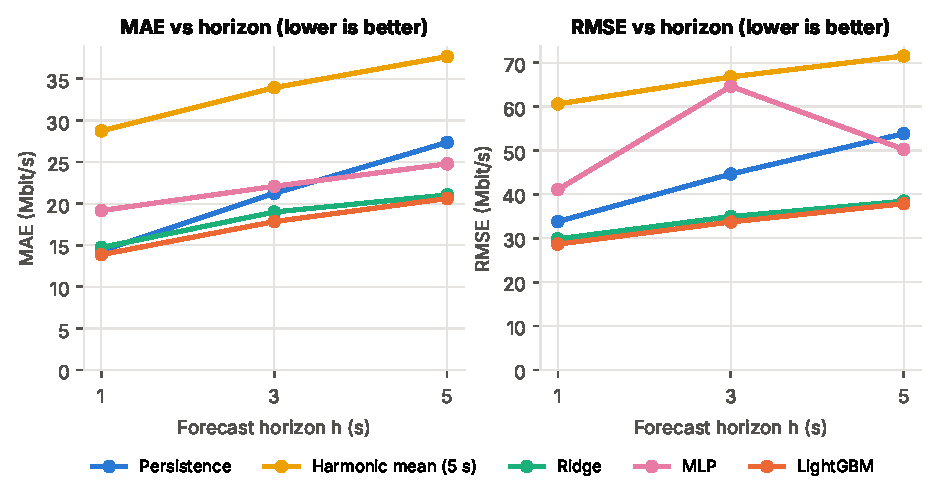
\includegraphics[width=0.78\textwidth]{fig/fig_horizon.pdf}
\caption{Error versus forecast horizon. All learned models gain on persistence as the
horizon grows; LightGBM is the best everywhere.}
\label{fig:horizon}
\end{figure*}

Static traces are easier to improve on than drives (Table~\ref{tab:mob}): at 3\,s,
LightGBM cuts the MAE by 23\,\% when static but by 8\,\% when driving, where throughput is
lower and changes are driven by handovers and technology switches. Fig.~\ref{fig:example}
shows a 5-minute excerpt of a held-out drive. Persistence follows the measured throughput
with a delay; LightGBM anticipates part of the recoveries but also overshoots at times,
because a squared-error model predicts the conditional \emph{mean} of a skewed distribution.

\begin{table}[t]
\caption{Error by condition at $h=3$\,s (Mbit/s)}
\label{tab:mob}
\centering\footnotesize
\begin{tabular}{@{}llccc@{}}
\toprule
Condition & Model & MAE & RMSE & $n$ \\
\midrule
\multirow{2}{*}{Driving} & Persistence & 15.36 & 37.67 & \multirow{2}{*}{13,606} \\
 & LightGBM & \textbf{14.17} & \textbf{30.75} & \\
\multirow{2}{*}{Static} & Persistence & 32.22 & 55.36 & \multirow{2}{*}{7,274} \\
 & LightGBM & \textbf{24.72} & \textbf{38.66} & \\
\bottomrule
\end{tabular}
\end{table}

\begin{figure*}[t]
\centering
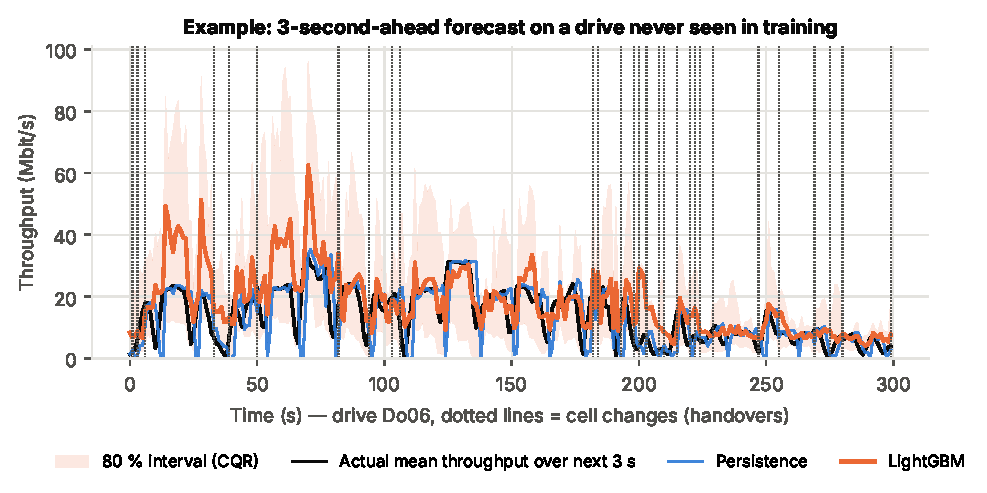
\includegraphics[width=0.85\textwidth]{fig/fig_example.pdf}
\caption{Five minutes of a drive never seen in training: actual mean throughput over the
next 3\,s, persistence, LightGBM and the CQR 80\,\% interval. Dotted lines mark cell
changes.}
\label{fig:example}
\end{figure*}

\subsection{What helps beyond history (Q2)}
\subsubsection{Ablation}
Fig.~\ref{fig:ablation} adds the feature groups one at a time. Over all test seconds,
\textbf{history alone is the best} (MAE 17.25); radio, mobility and space each add a little
error (17.51, 17.64, 17.84), a sign of mild overfitting with only 16 or 17 training drives
per fold. The picture changes right after a handover (1,447 seconds within 5\,s of a cell
change): the history-only model is \emph{worse than persistence} (15.27 vs 15.03), because
its features still describe the previous cell, while adding radio and mobility features
brings the error to 14.60, 3\,\% better than persistence. Context features matter exactly
where the past stops being informative. SHAP values~\cite{shap} on the deployed model
(Fig.~\ref{fig:shap}) agree: history accounts for 84\,\% of the total attribution, radio
8\,\%, space 5\,\% and mobility 3\,\%.

\begin{figure}[t]
\centering
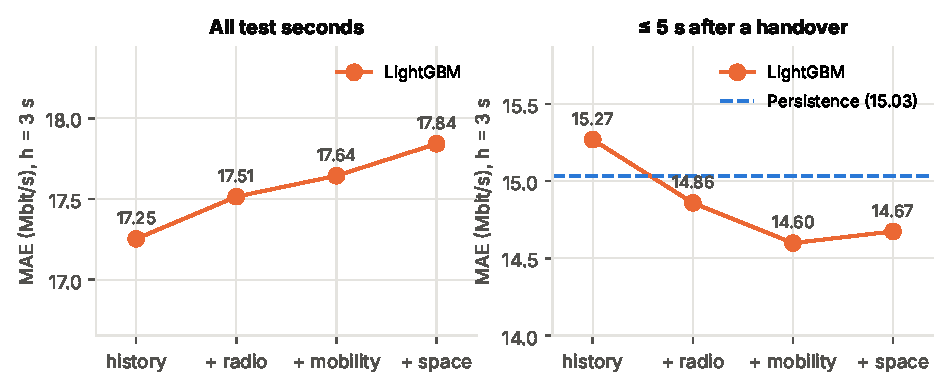
\includegraphics[width=\columnwidth]{fig/fig_ablation.pdf}
\caption{Cumulative ablation at $h=3$\,s. Left: all test seconds, history alone is best.
Right: within 5\,s after a handover, radio and mobility features are needed to beat
persistence.}
\label{fig:ablation}
\end{figure}

\begin{figure}[t]
\centering
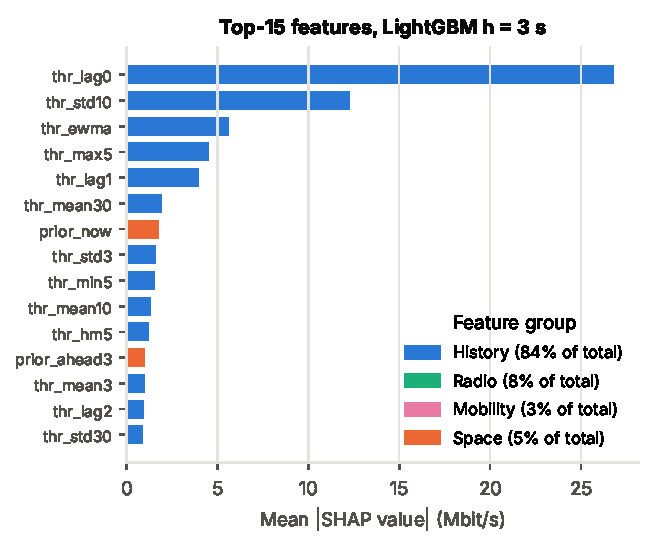
\includegraphics[width=0.85\columnwidth]{fig/fig_shap.pdf}
\caption{SHAP feature importance of LightGBM ($h=3$\,s). The current throughput and its
recent variability dominate; the space prior is the first non-history feature.}
\label{fig:shap}
\end{figure}

\subsubsection{Space}
The space-time prior is the most important non-history feature (Fig.~\ref{fig:shap}), but
it does not improve accuracy on held-out drives. This is not a coverage problem: 69 to
99\,\% of test points fall in a grid cell with a learned prior. The likely reason is that
throughput at a given place depends more on \emph{when} one passes (cell load, time of day,
whether the phone is on 5G or LTE) than on where: with 16 drives over ten weeks, the median
of past passes is a noisy estimate of the next one.

\subsubsection{Speed and Doppler}
If faster movement made the channel harder to predict, error would grow with speed. It
does not (Fig.~\ref{fig:speed}, left): the normalised MAE stays between 0.42 and 0.46 for
LightGBM, from walking pace to over 45\,km/h. Equation~(\ref{eq:doppler}) explains why: at
these speeds, $f_D$ stays below 300\,Hz and the coherence time is between 1.5 and a few
milliseconds. A 1-s measurement averages hundreds of coherence intervals, so the
fast fading that Doppler controls is invisible at this time scale. What does affect
predictability is large-scale change, i.e.\ handovers (Fig.~\ref{fig:speed}, right): the
error peaks 3 to 10\,s after a cell change and is lowest far from it.

\begin{figure}[t]
\centering
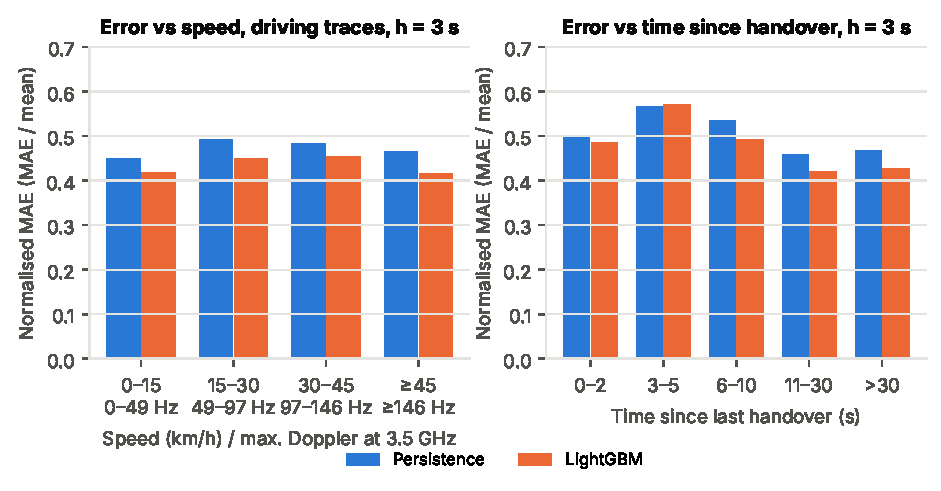
\includegraphics[width=\columnwidth]{fig/fig_speed_handover.pdf}
\caption{Normalised MAE (MAE divided by mean throughput) on driving traces at $h=3$\,s.
Left: error does not grow with speed or Doppler. Right: error peaks a few seconds after a
handover.}
\label{fig:speed}
\end{figure}

\subsection{Uncertainty (Q3)}
Uncalibrated quantile regression covers only 72.0\,\% of held-out targets with its nominal
80\,\% intervals (Table~\ref{tab:unc}). Conformal calibration raises coverage to
78.0\,\% (75.0 to 80.6\,\% per fold) for a 3\,\% wider interval. The remaining 2-point gap
is the price of non-exchangeable drives: calibration drives differ from test drives.
Intervals adapt to the situation (Fig.~\ref{fig:unc}): their median width is about 5\,Mbit/s
when a low throughput is forecast and above 100\,Mbit/s when it exceeds 50\,Mbit/s, which
matches the larger variability of high-throughput 5G.

\begin{table}[t]
\caption{80\,\% prediction intervals, $h=3$\,s}
\label{tab:unc}
\centering\footnotesize
\begin{tabular}{@{}lccc@{}}
\toprule
Method & Coverage & Range over folds & Width (Mbit/s) \\
\midrule
Quantile regression & 72.0\,\% & 69.1--75.6\,\% & 46.7 \\
CQR (calibrated) & \textbf{78.0\,\%} & 75.0--80.6\,\% & 47.9 \\
\bottomrule
\end{tabular}
\end{table}

\begin{figure}[t]
\centering
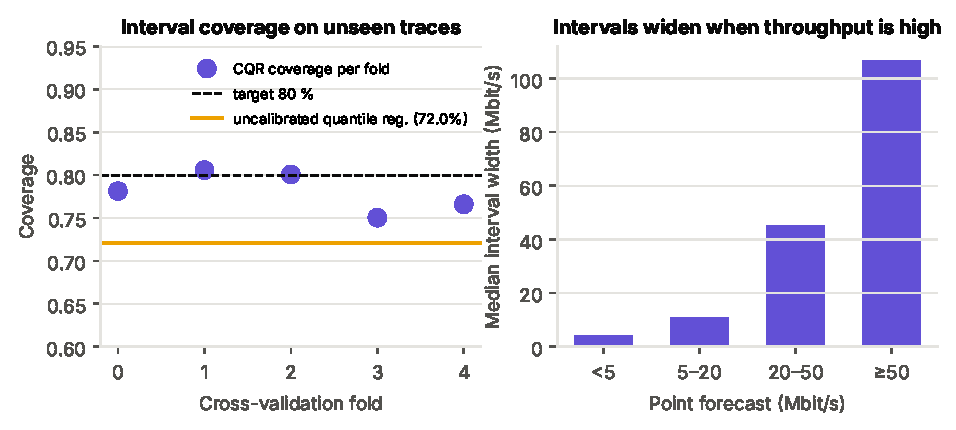
\includegraphics[width=\columnwidth]{fig/fig_uncertainty.pdf}
\caption{Left: CQR coverage per fold against the 80\,\% target and the uncalibrated
quantile regression. Right: interval width grows with the forecast level.}
\label{fig:unc}
\end{figure}

\begin{figure}[t]
\centering
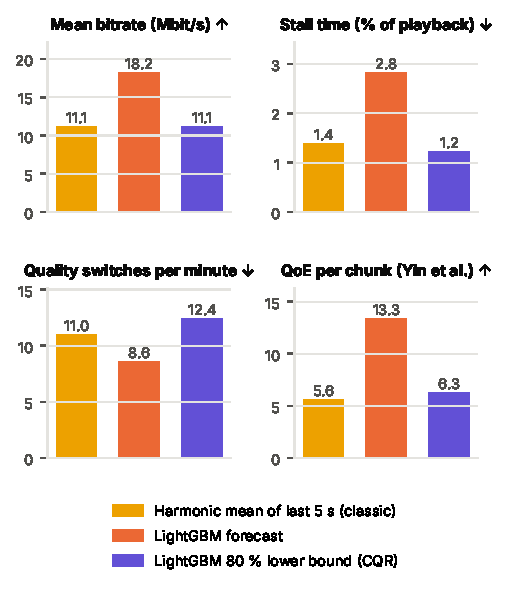
\includegraphics[width=0.95\columnwidth]{fig/fig_abr.pdf}
\caption{Trace-driven video streaming (mean over 21 traces, out-of-fold predictions).
The forecast raises bitrate and QoE; its calibrated lower bound minimises stalls.}
\label{fig:abr}
\end{figure}

\subsection{Video streaming (Q3)}
Fig.~\ref{fig:abr} reports the streaming simulation over the 21 traces. With the LightGBM
forecast, the player streams at 18.2\,Mbit/s on average instead of 11.1\,Mbit/s with the
harmonic mean, switches quality less often (8.6 vs 11.0 per minute), at the cost of more
stalls (2.8\,\% vs 1.4\,\% of playback). The QoE of Eq.~(\ref{eq:qoe}) rises from 5.6 to
13.3 per chunk, and is higher on \textbf{19 of the 21 traces}. Using the CQR lower bound
instead gives the fewest stalls (1.2\,\%) at the same mean bitrate as the harmonic mean,
and a higher QoE on 14 of 21 traces. The interval therefore offers a direct trade-off: the
point forecast maximises quality, while the lower bound is the safe choice for
stall-sensitive services.



% ================================================================== VI
\section{Discussion}
\label{sec:discussion}

\subsubsection{Beating persistence is the real test}
Persistence is a strong baseline at 1\,s and many published accuracies would look
modest against it. Reporting skill against persistence, on drives held out entirely, is
what makes the gains of 16 to 25\,\% at 3 and 5\,s credible.

\subsubsection{Space-time information: a negative result}
The idea that a vehicle can anticipate QoS from where it will be is appealing, and the
prior is the most used non-history feature, yet it does not reduce error here. Two
conditions would likely be needed: many more passes per location (so that the prior
captures the location effect rather than one day's load) and longer horizons, where the
current throughput says less about the future. Datasets from vehicle fleets, such as Berlin
V2X~\cite{berlinv2x}, are the natural next test.

\subsubsection{Physics sets the right time scale}
The absence of a speed effect is consistent with channel physics: Doppler governs
millisecond-scale fading, which 1-s KPIs average out. At the 1-to-5-s scale, mobility acts
through handovers and technology changes, and that is where context features help.

\subsubsection{Limitations}
One operator, one city and 21 download traces, collected in 2019--2020 on NSA 5G; the
carrier frequencies used for Doppler are assumed; the KPIs come from a phone application at
about 1\,Hz; hyperparameters were not tuned; the streaming simulator ignores TCP dynamics;
the real-time system was tested with a replayed drive, not inside an operator network.

% ================================================================== VII
\section{Conclusion}
\label{sec:conclusion}
On real 5G measurements and drives never seen in training, a gradient-boosted model
forecasts the throughput of the next 1 to 5\,s better than persistence in every fold, with
gains growing with the horizon (up to 25\,\% MAE and 30\,\% RMSE at 5\,s). History carries
most of the signal; radio and mobility indicators matter right after handovers; and a
space-time prior learned from other drives does not help on this dataset. Conformal
calibration brings the coverage of 80\,\% intervals from 72 to 78\,\%, and in a streaming
simulation the forecast more than doubles the quality of experience of the classic
estimator. The model runs as a real-time service with a Grafana dashboard and predictive
alerts. Future work: fleet-scale data for the spatial prior, longer horizons, 5G
standalone networks, and online re-calibration of the intervals.

% ================================================================== REFERENCES
\begin{thebibliography}{99}
\footnotesize
\setlength{\itemsep}{1pt}
\bibitem{5gaa} 5GAA Automotive Association, ``Making 5G proactive and predictive for the automotive industry,'' White Paper, Jan. 2020.
\bibitem{nwdaf} 3GPP, ``Architecture enhancements for 5G System (5GS) to support network data analytics services,'' TS 23.288.
\bibitem{linkforecast} C.~Yue, R.~Jin, K.~Suh, Y.~Qin, B.~Wang, and W.~Wei, ``LinkForecast: Cellular link bandwidth prediction in LTE networks,'' \emph{IEEE Trans. Mobile Comput.}, vol.~17, no.~7, pp.~1582--1594, 2018.
\bibitem{lumos5g} A.~Narayanan \textit{et al.}, ``Lumos5G: Mapping and predicting commercial mmWave 5G throughput,'' in \emph{Proc. ACM IMC}, 2020, pp.~176--193.
\bibitem{raca2020} D.~Raca, D.~Leahy, C.~J. Sreenan, and J.~J. Quinlan, ``Beyond throughput, the next generation: A 5G dataset with channel and context metrics,'' in \emph{Proc. ACM MMSys}, 2020, pp.~303--308.
\bibitem{yin2015} X.~Yin, A.~Jindal, V.~Sekar, and B.~Sinopoli, ``A control-theoretic approach for dynamic adaptive video streaming over HTTP,'' in \emph{Proc. ACM SIGCOMM}, 2015, pp.~325--338.
\bibitem{rappaport} T.~S. Rappaport, \emph{Wireless Communications: Principles and Practice}, 2nd~ed. Prentice Hall, 2002.
\bibitem{lightgbm} G.~Ke \textit{et al.}, ``LightGBM: A highly efficient gradient boosting decision tree,'' in \emph{Proc. NeurIPS}, 2017, pp.~3146--3154.
\bibitem{grinsztajn} L.~Grinsztajn, E.~Oyallon, and G.~Varoquaux, ``Why do tree-based models still outperform deep learning on typical tabular data?'' in \emph{Proc. NeurIPS Datasets and Benchmarks}, 2022.
\bibitem{cqr} Y.~Romano, E.~Patterson, and E.~Cand\`es, ``Conformalized quantile regression,'' in \emph{Proc. NeurIPS}, 2019.
\bibitem{vovk} V.~Vovk, A.~Gammerman, and G.~Shafer, \emph{Algorithmic Learning in a Random World}. Springer, 2005.
\bibitem{angelopoulos} A.~N. Angelopoulos and S.~Bates, ``A gentle introduction to conformal prediction and distribution-free uncertainty quantification,'' arXiv:2107.07511, 2021.
\bibitem{arp} D.~Arp \textit{et al.}, ``Dos and don'ts of machine learning in computer security,'' in \emph{Proc. USENIX Security Symp.}, 2022.
\bibitem{shap} S.~M. Lundberg and S.-I. Lee, ``A unified approach to interpreting model predictions,'' in \emph{Proc. NeurIPS}, 2017.
\bibitem{berlinv2x} R.~Hernang\'omez \textit{et al.}, ``Berlin V2X: A machine learning dataset from multiple vehicles and radio access technologies,'' in \emph{Proc. IEEE VTC2023-Spring}, 2023.
\end{thebibliography}

% ================================================================== APPENDIX
\appendix
\renewcommand\thesection{\Alph{section}}
\section{Code -- Method Mapping}
\begin{center}\footnotesize
\setlength{\tabcolsep}{3pt}
\begin{tabular}{@{}p{40mm}p{44mm}@{}}
\toprule
File & Role \\
\midrule
\texttt{src/qosf/data.py} & Download, 1-s grid, cleaning (§\ref{sec:data}) \\
\texttt{src/qosf/features.py} & Features, target (\ref{eq:target}), Doppler (\ref{eq:doppler}), prior (\ref{eq:deadreckoning}) \\
\texttt{src/qosf/models.py} & Baselines, ridge, MLP, LightGBM \\
\texttt{src/qosf/conformal.py} & CQR, Eq.~(\ref{eq:cqr}) \\
\texttt{src/qosf/abr.py} & Streaming simulator, QoE (\ref{eq:qoe}) \\
\texttt{scripts/run\_experiments.py} & All experiments of §\ref{sec:results} \\
\texttt{scripts/train\_final.py} & Deployable model \\
\texttt{realtime/} & API, replayer, Grafana (§\ref{sec:system}) \\
\texttt{tests/} & Leakage, target, Doppler, ABR, API tests \\
\bottomrule
\end{tabular}
\end{center}
Reproduction (from the repository root):
\begin{itemize}
\item \texttt{pip install -r requirements.txt}
\item \texttt{python scripts/run\_experiments.py}
\item \texttt{python scripts/train\_final.py}
\item \texttt{python scripts/make\_figures.py}
\item live demo: \texttt{docker compose up --build}, then \url{http://localhost:3000}
\end{itemize}

\end{document}
